\renewcommand{\NomeBloco}{Par Diferencial}
\renewcommand{\NomePTab}{tab_\NomeBloco}
\renewcommand{\NomeSTab}{tab_\NomeBloco2}
\renewcommand{\NomePFig}{fig_\NomeBloco}
\renewcommand{\NomeSFig}{fig_\NomeBloco2}
\renewcommand{\NomeTTab}{tab_\NomeBloco3}
\renewcommand{\NomeQTab}{tab_\NomeBloco4}

\subsection{\NomeBloco}

O bloco \NomeBloco{} tem a mesma fun{\c c}\~ao do bloco Comparador, por\'em apresenta uma topologia mais simples, j\'a que contem somente o primeiro est\'agio, chamado de "Par Diferencial". O bloco apresenta as defini{\c c}\~oes de sinais de entrada e sa\'ida referidos na \autoref{\NomeSTab}.

\begin{table}[htbp]
\caption{Sinais do bloco \NomeBloco}
\label{\NomeSTab}
\centering
\begin{tabular}{ccl}

    \toprule
    Sinal & Tipo    & Descri{\c c}\~ao        \\
    \midrule \midrule
    Vp (+) & Entrada & Entrada positiva do Comparador\\
    \midrule
    Vn (-) & Entrada & Entrada negativa do Comparador\\
    \midrule
    Ibias & Entrada & Corrente de polariza{\c c}\~ao do Comparador\\
    \midrule
    Vo & sa\'ida & Sa\'ida do Comparador\\
    \bottomrule
\end{tabular}
\legend{Fonte: Produzido pelo autor}
\end{table}

O circuito projetado para o bloco \'e demonstrado na \autoref{\NomePFig}.

\begin{figure}[htb]
 \label{\NomePFig}
 \centering
    \centering
    \caption{Circuito CMOS projetado para o bloco \NomeBloco} 
    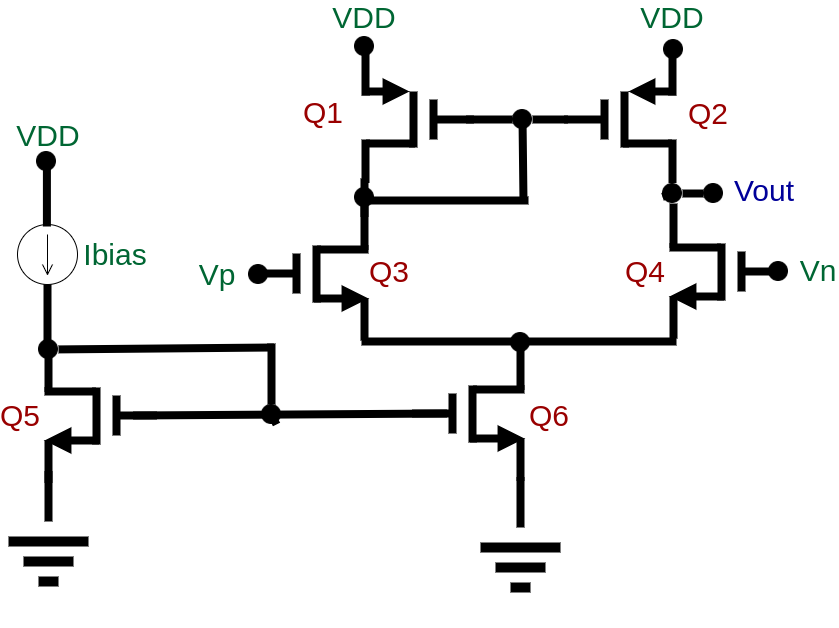
\includegraphics[scale=0.4]{Circuitos/diff_pair.png}
    \legend{Fonte: Produzido pelo autor}
\end{figure}

\begin{figure}[htb]
 \centering
    \centering
    \caption{Representa{\c c}\~ao em bloco do \NomeBloco} \label{\NomeSFig}
    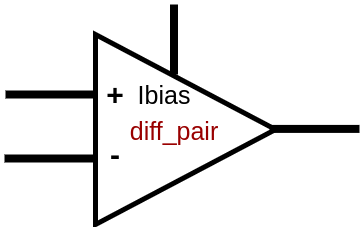
\includegraphics[scale=0.4]{Circuitos/diff_pair_block.png}
    \legend{Fonte: Produzido pelo autor}
\end{figure}

Os transistores utilizados no bloco \NomeBloco{} apresentam os par\^ametros mostrados na \autoref{\NomeTTab}.

\begin{table}[htbp]
\caption{Transistores do Bloco \NomeBloco}
\label{\NomeTTab}
\centering
\begin{tabular}{ccccc}
\toprule
Transistor & W ($\mu$m)  & L ($\mu$m)           & M (n° dispositivos) & S (n° dispositivos)\\
\midrule \midrule
Q1 e Q2 & 40 & 7 & 2 & 1\\
\midrule
Q3 e Q4 & 35 & 6 & 2 & 1\\
\midrule
Q5 e Q6¹ & 70 & 4 & 1 & 1\\

\bottomrule
\end{tabular}
\legend{Fonte: Produzido pelo autor}
\legend{$^1$Calculado de forma a produzir uma corrente de 50 $\mu$A}
\end{table}

Um segundo circuito, chamado de \emph{diff\_3} de mesma topologia apresentado na \autoref{\NomePFig} foi desenvolvido, por\'em com par\^ametros distintos, dados na \autoref{pard_diff3}.

\begin{figure}[htb]
 \centering
    \centering
    \caption{Representa{\c c}\~ao em bloco do diff\_3} \label{\NomeSFig}
    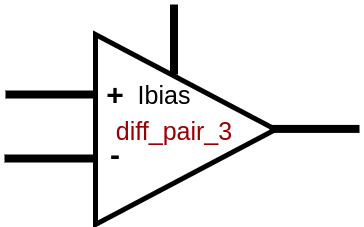
\includegraphics[scale=0.4]{Circuitos/diff_pair_3_block.png}
    \legend{Fonte: Produzido pelo autor}
\end{figure}

\begin{table}[htbp]
\caption{Transistores do Bloco diff\_pair\_3}
\label{pard_diff3}
\centering
\begin{tabular}{ccccc}
\toprule
Transistor & W ($\mu$m)  & L ($\mu$m)           & M (n° dispositivos) & S (n° dispositivos)\\
\midrule \midrule
Q1 e Q2 & 10 & 0.5 & 2 & 1\\
\midrule
Q3 e Q4 & 5 & 0.5 & 2 & 1\\
\midrule
Q5 e Q6¹ & 50 & 3 & 2 & 1\\

\bottomrule
\end{tabular}
\legend{Fonte: Produzido pelo autor}
\legend{$^1$Calculado de forma a produzir uma corrente de 50 $\mu$A}
\end{table}
\clearpage